\chapter{Protocol Implementation}
\section{Application Overview}
To run this protocol in a practical scenario, at least 3 different devices are required - one be Alice, one be Bob and one be Courier. This application implements all 3 entities within it, so once the device has this application, it can be any entity in the protocol. To achieve this, at the start of the application, user is asked to choose a particular role for the device to be. There are 4 options:
\begin{enumerate}
\item \textbf{DataCreator}, who creates message and wants to send it out.
\item \textbf{CourierReciever}, who connects to DataCreator and receives the message from it.
\item \textbf{DataReceiver}, who is the recipient of DataCreator.
\item \textbf{CourierSender}, who possesses the message from DataCreator and should transmit it to DataReceiver.
\end{enumerate}
Once the choice has been made, the graphical user interface will adjust to the selected role, and user will be requested to input some information related to the selected role. \par
Below is a snapshot of the GUI of the application, it shows all the selections and textfields that will be used when the application interacts with user.

\begin{figure}[h!]
\centering
\includegraphics[width=0.8\textwidth,natwidth=818,natheight=722]{figures/guiall.png}
\caption{GUI Overview}
\end{figure}

To run Submit Protocol, Alice should choose to run as DataCreator and Courier should choose to run as CourierReceiver. Then Courier transports to Bob and chooses to run as CourierSender, meanwhile Bob should choose to run as DataReceiver to run Transmit Protocol with Courier. The detailed instruction of how to run those two sub-protocols is given in the appendix. \par

To further illustrate how user can interact with the system, a use case diagram is given and every use cases appear in the diagram will be explained. For disambiguating, the ``Alice", ``Bob" and ``Courier" appeared in the use case diagram do not mean the protocol entity as introduced in the system model, but are the names of the actors who control the device. The name of the actor simply reflects which entity the actor wants to be in the protocol. \\

\begin{figure}[h!]
\centering
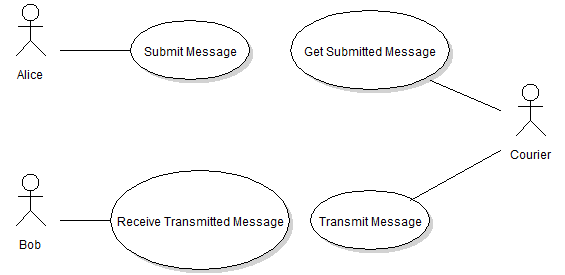
\includegraphics[width=0.6\textwidth,natwidth=565,natheight=275]{figures/usecasediagram.png}
\caption{Use Case Diagram}
\end{figure}

\subsection*{Use Case 1: Submit Message}
\begin{tabular}{|l|p{0.6\textwidth}|}
 \hline
 Title & Submit Message \\ \hline
 Primary Actor & Alice \\ \hline
 Goal in Context & Alice tries to submit the message to a Courier \\ \hline
 Scope & System (Black Box) \\ \hline
 Level & \\ \hline
 Stakeholders & Alice and Courier \\ \hline
 Success Guarantees & Message is received by Courier and Alice confirms the fact \\ \hline
 Trigger & Alice starts the Submit Protocol \\ \hline
 Main Success Scenario & 
 \parbox{9cm}{
  \medskip
  1. Alice starts the application. \\
  2. Alice selects ``DataCreator" as the protocol entity in the application. \\
  3. Alice specifies all related information as instructed in the ``Run Submit Protocol" section in Appendix A: User Manual. \\
  4. Alice starts running the protocol.
  \medskip
 }
 \\ \hline
\end{tabular}
\\
\\
\subsection*{Use Case 2: Get Submitted Message} 
\begin{tabular}{|l|p{0.6\textwidth}|}
 \hline
 Title & Get Submitted Message \\ \hline
 Primary Actor & Courier \\ \hline
 Goal in Context & Courier tries to obtain the message of Alice \\ \hline
 Scope & System (Black Box) \\ \hline
 Level & \\ \hline
 Stakeholders & Courier and Alice \\ \hline
 Success Guarantees & Courier gets a message from Alice \\ \hline
 Trigger & Courier starts the Submit Protocol \\ \hline
 Main Success Scenario & 
 \parbox{9cm}{
  \medskip
  1. Courier starts the application. \\
  2. Courier selects ``CourierReceiver" as the protocol entity in the application. \\
  3. Courier specifies all related information as instructed in the ``Run Submit Protocol" section in Appendix A: User Manual. \\
  4. Courier starts running the protocol.
  \medskip
 }
 \\ \hline
\end{tabular}
\\
\\
\subsection*{Use Case 3: Receive Transmitted Message} 
\begin{tabular}{|l|p{0.6\textwidth}|}
 \hline
 Title & Receive Transmitted Message \\ \hline
 Primary Actor & Bob \\ \hline
 Goal in Context & Bob tries to receive message of Alice carried by Courier \\ \hline
 Scope & System (Black Box) \\ \hline
 Level & \\ \hline
 Stakeholders & Bob and Courier \\ \hline
 Success Guarantees & Bob receives the message \\ \hline
 Trigger & Bob starts the Transmit Protocol \\ \hline
 Main Success Scenario & 
 \parbox{9cm}{
  \medskip
  1. Bob starts the application. \\
  2. Bob selects ``DataReceiver" as the protocol entity in the application. \\
  3. Bob specifies all related information as instructed in the ``Run Transmit Protocol" section in Appendix A: User Manual. \\
  4. Bob starts running the protocol.
  \medskip
 }
 \\ \hline
\end{tabular}
\\ 
\\
\subsection*{Use Case 4: Transmit Message}
\begin{tabular}{|l|p{0.6\textwidth}|}
 \hline
 Title & Transmit Message \\ \hline
 Primary Actor & Courier \\ \hline
 Goal in Context & Courier tries to transmit Alice's message to Bob \\ \hline
 Scope & System (Black Box) \\ \hline
 Level & \\ \hline
 Stakeholders & Courier and Bob\\ \hline
 Success Guarantees & Message is received by Bob and Courier confirms the fact \\ \hline
 Trigger & Courier starts the Transmit Protocol \\ \hline
 Main Success Scenario & 
 \parbox{9cm}{
  \medskip
  1. Courier starts the application.
  2. Courier selects ``CourierSender" as the protocol entity in the application.
  3. Courier specifies all related information as instructed in the ``Run Transmit Protocol" section in Appendix A: User Manual.
  4. Courier starts running the protocol.
  \medskip
 }
 \\ \hline
\end{tabular}
\\

\section{Software Design}
The implementation of this protocol mainly consists of two parts - a core library and an user interface. The core library defines the framework of the program and provides all essential components for running the protocol. While the user interface takes user's input, configures components provided by the core library, runs the protocol and outputs running results if necessary. This design separates the implementation of user interfaces from the actual running of the protocol, the major benefit is that when this protocol is running on different devices or platforms, its user interfaces can be customized and easily plugged to the core library without modifying it.

\subsection{Program Architecture}
As introduced above, the whole program contains 4 roles - DataCreator, DataReceiver, CourierSender and CourierReceiver. Classfied by their main structure, those 4 different roles fall into 2 categories - (1) Accepter, who continuously listens to the port and waits for incoming connection. (2) Initiator, who actively connects to a Accepter. Although these two categories sounds similar to Client-Server pattern, it is not quite the case because Accepter does not actually provide any service. Based on their behaviour definition in protocol specification, DataCreator and DataReceiver belong to Accepter, while CourierSender and CourierReceiver belong to Initiator. Following paragraphs will introduce the internal architecture for Accepter and Initiator respectively.
\paragraph{Accecpter}
Accepter contains 5 main parts:
\begin{itemize}
\item Dispatch Thread \\
The Dispatch Thread listens to the program port, waits for incoming connections. Once it receives a connection, it will create a new session, then handover the connection to the newly created session. After that, it will continue listening to the port, wait for next incoming connection.

\item Sessions \\
Sessions are created by the Dispatch Thread, each session corresponds to a single connection and sessions are independent between each other. Once a session takeovers a connection, it is fully responsible for it. Inside a session there is a Delegate and a Sub-thread. 
\par The \textbf{Delegate} defines all communication content (e.g. a Delegate of Alice defines the content of messages to send out, and it also defines what to do when receives a certain message), it behaves like a state machine which takes message as input, processes the message and output a new message for response. During the processing of input messages, it may interact with the 3 global objects - User Interface, Cryptographic Kit and Data Manager. The detail of Delegate will be explained in Delegate Model.
\par The \textbf{Sub-thread} listens to the connection which is handover by Dispatch Thread, capture any message from the connection. It delivers the captured message to Delegate, and receives a new message from Delegate. If the output message from Delegate does not indicate an exception or termination, the Sub-thread sends the message through the connection, otherwise it reports an error or terminates.

\item User Interface \\
The User Interface is shared between all sessions in Accepter. It displays all relative information to show the progress of the protocol running and reports errors to the user.

\item Cryptographic Kit \\
The Cryptographic Kit is shared between all sessions in Accepter. It provides functionalities of all cryptographic operations that is needed in the protocol, such as encryption, decryption, key generation, MAC generation and verification, and digital signature generation and verification. When any session need to do cryptographic operations, it just call from Cryptographic Kit and doesn't care the internal implementation. For the consistency concern, it is required that any two communicating device should use same Cryptographic Kit.

\item Data Manager \\
The Data Manager is shared between all sessions in Accepter. It keeps record of all data files in the device's disk which is related to the protocol, such as files of public keys, secret keys, and the message Courier carries. Data Manager is configured at the start of the application, when any session need data in disk, it just request from Data Manager.
\end{itemize}
The relation between those 5 components is illustrated in the figure ``Accepter Architecture".

\begin{figure}[h!]
\centering
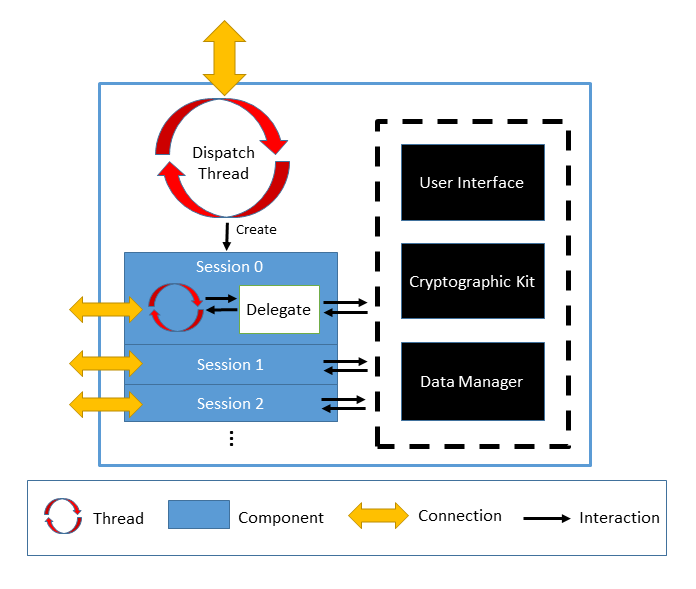
\includegraphics[width=\textwidth,natwidth=696,natheight=589]{figures/accepterarchitecture.png}
\caption{Accepter Architecture}
\end{figure}

\paragraph{Initiator}
Similar to Accepter, Initiator consists of 4 main parts: (1) Session, (2) User Interface, (3) Cryptographic Kit and (4) Data Manager. The major difference between Initiator and Accepter is that Initiator does not have a Dispatch Thread, every Initiator only has one Session. The Session is created once the Initiator is started, and it will ask its Delegate for a ``initial message" - which will be the first message of the protocol, and will be sent to the specified Accepter. The architecture design of Initiator is a simpler version of Accepter's, and it is illustrated in the figure ``Initiator Architecture".

\begin{figure}[h!]
\centering
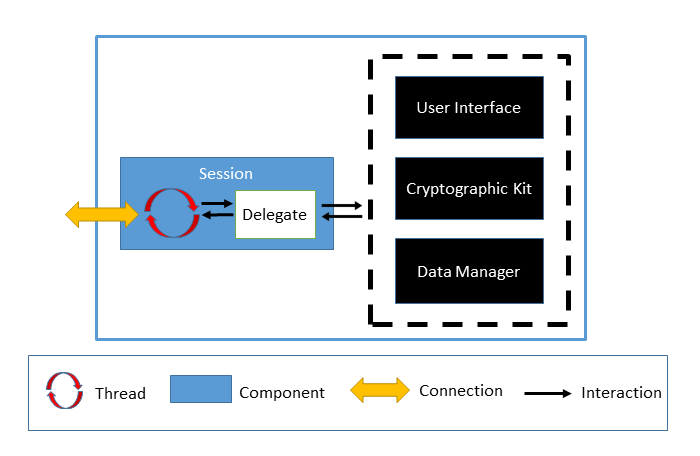
\includegraphics[width=\textwidth,natwidth=700,natheight=456]{figures/initiatorarchitecture.png}
\caption{Initiator Architecture}
\end{figure}

\subsection{Delegate Model}
The object Delegate is the essence of the application, it directly refers to the specification of the protocol, defines how an entity processes a message - here ``process a message" may involve doing cryptographic operations, checking message content validity and giving a response message.

Basically, every Delegate acts like a finite-state machine, who possesses an internal state, takes messages as inputs and outputs new messages as response. The internal state controls the behaviour of the Delegate - Delegates in different states will respond differently to a same input. So when an input message comes, Delegate will process the message according to its current state, if the message is successfully processed, it will change its current state and wait for next message, until it reaches the final state. 

Taking entity $\mathcal{A}$ as example,the figure below shows a 4-internal-state machine which abstracts the behaviour of $\mathcal{A}$: initially $\mathcal{A}$ is in Wait state, waiting for the first message. Once it receives the first message, it will process the message (according to the Submit Protocol, it will check the first message and submit its data to Courier). If $\mathcal{A}$ successfully processed M$_0$, it enters Submitted state, waiting for the second message. Then it will receive and process M$_1$ (according to the Submit Protocol, it will check the validity of the MAC).  If it is successful again, it enters the final state Checked and stops. If any error occurs in processing the input messages in early states, $\mathcal{A}$ directly enters final state Error and stops.

\begin{figure}[h!]
\centering
\includegraphics[width=0.8\textwidth,natwidth=585,natheight=352]{figures/statemachinefigure.png}
\caption{State Machine of $\mathcal{A}$}
\end{figure}

\subsection{Message Structure}
Based on the protocol specification, there are totally 5 different kinds of messages to exchange in a single success protocol run - 3 messages are needed to achieve Submit Protocol and 2 messages are needed to achieve Transmit Protocol. The design of message structure attempts to maximize the time efficiency of the protocol, thus no extra message will be exchanged and the lengths of messages will be minimized. All messages exchanged in this protocol are concatenations of 6 different kinds of primary blocks:
\begin{itemize}
\item \textbf{Integer Block} \\
Integer Block simply contains a single Integer, it occupies 4 bytes (based on the current JAVA's Implementation).

\item \textbf{MAC Block} \\
MAC Block contains a cryptographic MAC, whose size is defined by the Cryptographic Kit the application uses.

\item \textbf{Asymmetric Cipher Block} \\
Asymmetric Block contains an asymmetric cipher. Because encrypting a long plaintext using asymmetric encryption takes long time, to reduce the computational consumption, the length of plaintext for asymmetric encryption is restricted in this protocol, so that only one cipher block will be produced after the encryption. As the consequence, the size of Asymmetric Cipher Block is fixed, which is 128 bytes (based on a key of size 128 bits).

\item \textbf{ID Block} \\
ID Block contains two parts. The front part is a single byte which indicates the total length of the ID string and the following part is a string of characters representing the ID. The size of ID Block is variable, which is the length of ID string plus 1 bytes.

\item \textbf{Meta Block} \\
The Meta Block in application design is different with ``Meta block" in protocol specification. It contains a concatenation of 3 parts - (1) an integer indicates the size of the rest of this Meta Block, (2) an asymmetric cipher of the meta of the message, (3) a symmetric cipher of the signature of the meta. As explained in Asymmetric Cipher Block, the size of all asymmetric ciphers is fixed, so the size of the asymmetric cipher is (size of Meta Block - size asymmetric cipher).

\begin{figure}[h!]
\centering
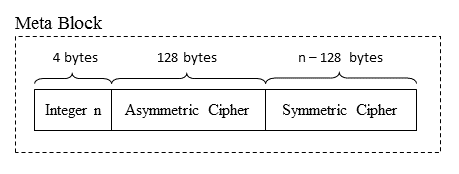
\includegraphics[width=0.6\textwidth,natwidth=459,natheight=174]{figures/metablock.png}
\caption{Structure of Meta Block}
\end{figure}

\item \textbf{Message Block} \\
The Message Block is also different with ``Msg block" in protocol specification. Similar to Meta Block, it is the concatenation of 3 parts - (1) an integer indicates the size of the rest of this Message Block, (2) a symmetric cipher of the actual message content, (3) a MAC of the part (2). The size of symmetric cipher can also be deduced as the size of MAC is fixed.

\begin{figure}[h!]
\centering
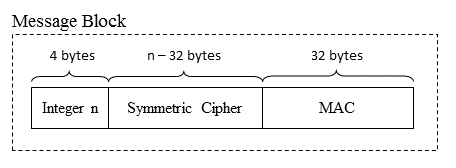
\includegraphics[width=0.6\textwidth,natwidth=456,natheight=168]{figures/messageblock.png}
\caption{Structure of Message Block}
\end{figure}
\end{itemize}

To summarize, 3 of these 6 primary blocks are fixed-size blocks (Integer Block, MAC Block and Asymmetric Cipher Block), while other 3 of them are variable-size blocks (ID Block, Meta Block and Message Block). All the messages exchanged in the protocol are constructed by these primary blocks through concatenation, and they will be illustrated below.

\subsubsection*{Submit Protocol}
Message 1, from Courier to Alice: \\
\begin{tabular}{|c|c|c|}
 \hline
 ID Block & Integer Block & \qquad\; AC Block \qquad\; \\ \hline
\end{tabular}

\noindent\bigskip
\textit{Note that ``AC Block" denotes Asymmetric Cipher Block.}

\noindent
Message 2, from Alice to Courier: \\\bigskip
\begin{tabular}{|c|c|c|c|c|}
 \hline
 ID Block & ID Block & \qquad\; Meta Block \qquad\; & 
 \quad\, Message Block \quad\, & MAC Block \\ \hline
\end{tabular}

\noindent
Message 3, from Courier to Alice: \\\bigskip
\begin{tabular}{|c|c|c|}
 \hline
 MAC Block \\ \hline
\end{tabular}

\subsubsection*{Transmit Protocol}
Message 1, from Courier to Bob: \\
\begin{tabular}{|c|c|c|c|c|c|}
 \hline
 ID Block & \qquad\; AC Block \qquad\; & 
 \; Meta$_0$ \; & Message$_0$ & 
 \; Meta$_1$ \; & Message$_1$
 \\ \hline
\end{tabular}
\textbf{......} \\
\noindent\bigskip
\textit{Multiple Meta Blocks and Message Blocks can be appended here.}

\noindent
Message 2, from Bob to Courier: \\\bigskip
\begin{tabular}{|c|c|c|}
 \hline
 MAC Block \\ \hline
\end{tabular}

\subsubsection*{Error Message Flag}
There are two kinds of messages exchanged in the protocol, all above messages are one of them, called Normal Message, the others called Error Message. Those two kinds of messages are distinguished by an Error Message Flag, which is the first byte of the message. Thus there is an extra step before above Normal Messages to be sent - they should be wrapped by an extra byte 0 at the front of them. While an Error Message contains two parts - (1) a byte indicates the size of the rest of the message, (2) a string of error information. As consequence, all messages start with a byte 0 will be treated as Error Message. The figure below further illustrates the difference between Normal Message and Error Message.

\begin{figure}[h!]
\centering
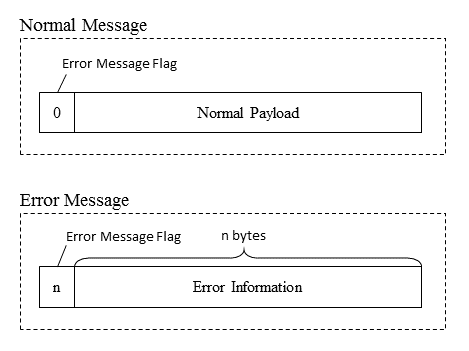
\includegraphics[width=0.6\textwidth,natwidth=469,natheight=351]{figures/normalvserrormessage.png}
\caption{Normal Message and Error Message}
\end{figure}

\section{Implementation Details}
\subsection{UML Class Diagram}
A UML Class Diagram has been plotted to show all the main classes in the program and the relations between them.
\begin{figure}[h!]
\centering
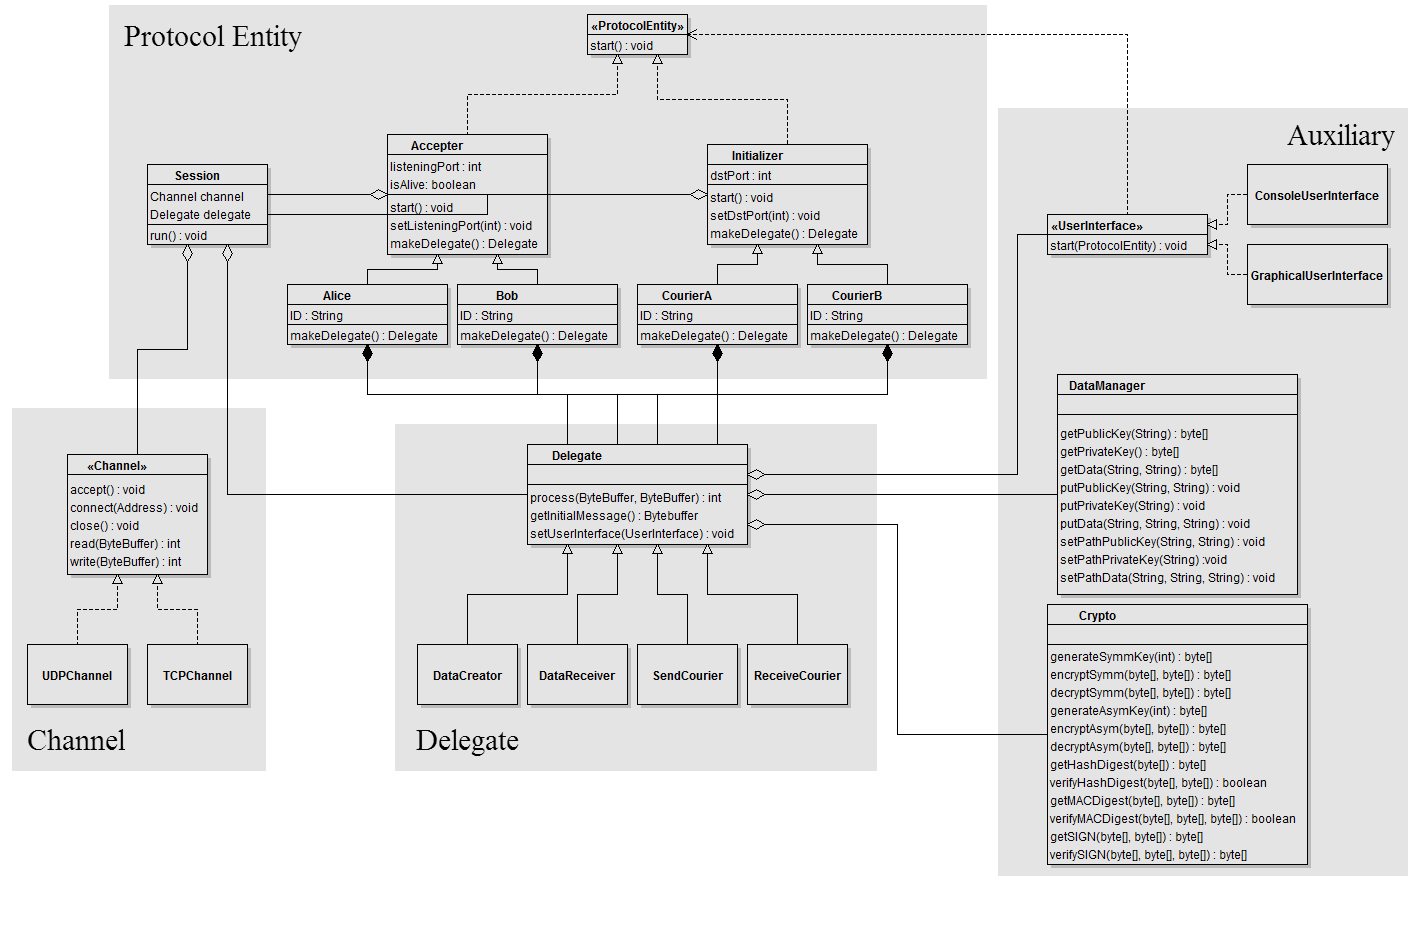
\includegraphics[width=\textwidth,natwidth=1416,natheight=935]{figures/umldiagram.jpg}
\caption{UML Diagram}
\end{figure}

According to the diagram, the whole program can be separated into 4 main parts:
\begin{itemize}
\item \textbf{Protocol Entity} \\
This part defines the framework of this application. Any protocol entity can be first specified into an Accepter or an Initiator, then based on the role it plays, it can be further classified into a particular role like Alice, Bob, CourierA (Courier who connects to Alice) or CourierB (Courier who connects to Bob). As shown in the diagram, every level of classification corresponds to a group of classes and lower level classes inherit from the higher level classes. The main job of Protocol Entity classes is creating, initializing and managing its Session objects. While a Session class - which is possessed by every protocol entity, deals with the message transmission issues for the entity, such as requesting next messages from Delegate, sending messages to the Channel, etc.

\item \textbf{Channel} \\
The Channel is used in Session class, it is an Interface denotes a place where messages can be sent and received. Ideally, when two channels are connected, devices can easily push message in and receive message from their channels without awareness of any detail about the connection. However, due to different networks and protocols suites may be used when running CDSProtocol, various implementations of Channel are necessary. As shown in the diagram, possible implementations of Channel Interface can be TCPChannel and UDPChannel, corresponds to connecting under TCP or UDP. Except above two, even more different channels could be developed like BluetoothChannel, CableChannel, etc. In this prototype program, only UDPChannel is currently implemented and the detail of it will be explained in the later ``Connection Establishment" section.

\item \textbf{Delegate} \\
As has been demonstrated in the ``Delegate Model", Delegate class defines the ``rule" of an entity. It takes a message as input, processes the message and outputs a responding message if there is one. However, Delegate is just an abstract notion, its children classes define the real ``rules" of each entity respectively. As shown in the diagram, DataCreator, DataReceiver, CourierSender, CourierReceiver are 4 different implementations of Delegate class, they define the ``rules" for the 4 entities correspondingly - Alice, Bob, CourierA and CourierB.

\item \textbf{Auxiliary} \\
This part contains 3 components that can be totally independent with the design of CDSProtocol. The UserInterface only deals with inputs from user and displays output to user. Reflect to the software design, its implementation can be various to fit different devices and platforms. The DataManager takes charge of managing the disk files that is related to the running of the protocol. And the Crypto represents ``Cryptographic Kit" in the software design, its job is to provide all cryptographic operations that is needed in the protocol.
\end{itemize}

\paragraph{Extensibility and Reusability}
The design of the program structure attempts to maximize the extensibility and reusability of the program in order to make the program easy for modifying and extending after release. It should be noticed that all components of the program are loosely coupled which makes them easy for reuse, and frequently used inheritance and interfaces makes the program extensible. Developers can modify or create their own entities, delegates, channels or even cryptographic kits without affecting other parts of the code. 

\subsection{Connection Establishment}
The Channel is used to establish connections between entities in program. Each Channel object is associated with a local address and listening port before connected. There are 2 steps for two entities to get connected using Channel. Firstly, Initiator initiates the connection by calling the connect() method of its Channel object, specifying the destination IP address. Then the Accepter accepts the connection by calling the accept() method of its Channel object. The accept() method will wait until there is a connection to accept and what it really does is creating a new Channel object which is connected to the incoming connection, and returns that newly created Channel object. Once the connection is accepted, both entities can use Channel's read() and write() method for receiving and sending messages. If any of the entity chooses to terminate the connection, it calls the close() method of its Channel, then both Channels are closed.

\paragraph{UDPChannel}
The above connecting mechanism is effective in this protocol, as the Channel object who accepts connections will not be connected to any Channel, thus it can accept several connections without changing its listening port - imaging if channel gets connected once it accepts a connection, then when a new connection comes, it will not be able to accept it. However, to implement this mechanism for UDP requires extra effort because UDP itself is connectionless and every packet sent or received is independent between each other. The real process for establishing connections using UDPChannel is: When the Initiator calls the connect() method of its Channel object, the channel records the destination address and port number but sends nothing. So when Accepter calls accept() nothing will happen until Initiator sends the first message, at which point accept() will create a new Channel object with a different listening port and all future messages will be sent through this Channel object. So, when Accepter sends back the second message, the port number of the channel sending the message is different with what Initiator specified in the first message. So when Initiator receives a reply message fron Accepter, it changes its channel's destination port number to the coming channel's port number, so that its future messages will be sent to the Accepter's newly created channel. Finally the connection is built between Initiator's channel and Accepter's newly created channel.

\subsection{Message Processing}
When a message is received from the channels, it will be examined by the session first, where the Error Message Flag will be checked. If the Error Message Flag (the first byte of the received message) is greater than 0, it indicates the message is an Error Message and the number of the Error Message Flag represents is the length of the error information. Then session will extract the error information and displays it on the user interface. If the Error Message Flag is 0, it means the message is a Normal Message. Then session will extract the payload and feed it to the delegate. Delegate will further process the payload and returns an integer indicating the size of the responding message. If the integer is 0 it means the message is successfully processed and no further messages to be sent. If the integer is negative, it means an exception occurs during the processing.

When session gets a message from delegate, it should wrap it into a Normal Message by adding a 0 byte in the front of the message. Then session sends the wrapped message to the channel and waits for receiving next message from the channel.

\subsection{Cryptographic operations}
The cryptographic functions provided by the Crypto class in this program are mainly built from two Java packages ``java.security" and ``javax.crypto", thus the security of this application highly relies on the implementation inside those two Java packages. Below will list and explain all the cryptographic operations used in this protocol. As there is no sign indicating there is any flaw inside the Java security packages, we will not dig too deep into the security cryptographic implementation. 

\begin{itemize}
\item \textbf{Symmetric Encryption / Decryption / KeyGeneration} \\
The symmetric encryption / decryption scheme used is AES \cite{Miller}. The mode of operation used is CBC \cite{ehrsam1978message}. The padding scheme is PKCS\#5 \cite{RFC2898}. The size of key used is 128 bits and it should not exceed 936 bits.

\item \textbf{Asymmetric Encryption / Decryption / KeyGeneration} \\
The asymmetric encryption / decryption scheme used is RSA. The mode of operation used is ECB, however, for efficiency concern, the size cipher block of asymmetric encryption will be restricted to 1, so mode of operation will not actually be used in the program. Th padding scheme is PKCS\#1 \cite{RFC2313}. The size of key used is only 1024 bits, as this is only a prototype application and key size can easily be increased in future.

\item \textbf{MAC Creation / Verification} \\
The MAC algorithm used is Hmac-SHA-256 \cite{RFC6234}. The size of key used is same to symmetric encryption / decryption, which is 128 bits.

\item \textbf{Digital Signature Creation / Verification} \\
The signature algorithm used is RSA. The cryptographic hash function used in SHA256 \cite{RFC6234}. They key size is same to asymmetric encryption / decryption, which is 1024 bits.
\end{itemize}

\subsection{File Management}
It is assumed that adversary is not able to hack into its target entity's system, that is, the adversary can not access to the memory or disk of a honest entity's device. Based on this assumption, all the data files are stored explicitly in device's disk.
\paragraph{Keys}
As a single device is able to act as several different entities, it is possible that one device possesses several secret keys and presumably a long list of others' public keys. The user should take care of his/her own key files, and before the protocol starts, he/she specifies the locations of all keys. Then during running, the application will read those files when necessary.
\paragraph{Alice's Message Content}
Similar to the keys, Alice's message content should be stored in the disk of Alice's device. Before the start of the protocol, user will be requested to specify the location of that file. Then during Submit Protocol, the file will be read when necessary.
\paragraph{Courier's Payload}
Courier's payload files are not specified by user, it is managed by the application. For every Courier entity, it has a working directory, by default, Courier's working directory is in the application's directory, named after its ID. Once Courier gets data from Alice in Submit Protocol, it will save the data into its working directory, the file name will be the destination entity's ID. For example, if Courier0 receives data from Alice to Bob, the data will be saved in the file ``./Courier0/Bob". As Courier may receives data from multiple datacreators, all further data will be appended to the file named after the receiver's ID, if no such file, program will create it. So, after the Message Acquisition phase, Courier may have several data files, and each contains data from multiple datacreators. Finally in Transmit Protocol, Courier transmits the corresponding data file to its destination entity base on the file name.

\subsection{Error Handling}
In this application, errors are classified into 4 main classes - user input error, I/O error, protocol error and timeout. Below will explain the details of these 4 errors and how they are handled in the program.
\paragraph{User Input Error}
User input errors occur when user input meaningless content into the application's textfield, such as inputing non-numeric string as port number, etc. This kind of errors will be caught before the protocol starts running, after user click ``Start" button. Once user input error is detected, its detail will be sent to user interface where the error detail will be shown to the user.
\paragraph{I/O Error}
I/O error denotes errors happening when reading/write files or sending/receiving through network channels, such as files not found when reading files, or port number is in use when creating a network socket, etc. These errors are caught during the running of the protocol and will cause termination of the protocol run. Similar to user input error, once I/O error is detected, its detail will be sent to user interface and then be shown to the user.
\paragraph{Protocol Error}
Protocol error is produced by the protocol itself, when there is some checking violation happens such as verifying a MAC to false, or the message size exceeds the capacity of Courier's storage, etc. All the checking processes have been fully described in the protocol specification, and the program strictly follows those processes. Because all checking operations happen in delegates while delegates processing the received messages, the protocol error is detected by delegates. Once a protocol error is detected, firstly, the error detail will be sent to user interface and be shown to the user. Meanwhile, the delegate will return a negative integer indicating error happens during processing. Then session will send a Error Message to the other entity reporting the error. However, for the security concern, Error Message will not include any detail about the error, currently it just carries a string ``Protocol Error".
\paragraph{Timeout}
Technically timeout is not an error but a mechanism of protecting an entity from waiting responses for too long time. And it is essential in this protocol because when an I/O error occurs during the protocol, it immediately terminates the program in this device, without reporting anything to the other device which still waits for reply. Timeout allows the other device to abort the protocol if no message is received after waiting for a certain amount of time. Timeout is detected in sessions. After sending out a message session will first check whether it is the end of the protocol, if it is, session will close the channel and terminate. If it is not, session will monitor the channel with a timer. Upon the time runs out, it will voluntarily close the channel and terminate.